
\documentclass[12pt,a4paper]{article}

\usepackage[dutch]{babel}
\usepackage[utf8]{inputenc}
\usepackage{hyperref}
\usepackage{graphicx}
\usepackage{float}
\usepackage{listings}


% Font
\renewcommand{\familydefault}{\sfdefault}

% Title Page
\title{Requirements Engineering: League of Legends eSports}
\author{Bellemans Jonah \and Caerts Stijn \and Dimova Yana \and Lambrichts Midas \and Verhoest Elise \and Vos Pieter}
\date{\today}


\begin{document}
	\pagenumbering{gobble}
	\maketitle
	\newpage
	\pagenumbering{arabic}
	\tableofcontents
	\newpage
	\section{Motivatie sportkeuze}
		We opteerden om e-sports, meer bepaald de ``League of Legends World Championships (LoL Worlds)'', te kiezen als sporttak voor dit project. Wij kozen hiervoor omdat deze sporttak origineel is, en een zeer duidelijke afbakening van de spel- en wedstrijdreglementen voorziet. Aangezien de meerderheid van de groepsleden vanuit een computer science-gerelateerde achtergrond komt, is de e-sport goed door de leden gekend, en is iedereen gemotiveerd om hieraan te werken.
	\section{Beschrijving Competitie}
		\subsection{Plaatsingsmatches}
			Teams plaatsen zich voor de competitie door middel van plaatsingswedstrijden die vroeger in het seizoen plaatsvinden. Voor elke regio (West-Europa, Noord-Amerika, Korea,\dots) worden een aantal ``Seeds'' vrijgehouden, die worden ingevuld door de beste ploegen van die regionale competities. De absolute topploegen van de wereld, zoals winnaars van eerdere jaren, kunnen via een ``wildcard'' rechtstreeks uitgenodigd worden voor deelname door het organisatorisch comité.
		\subsection{Wedstrijdverloop}
			Elke wedstrijd van het spel League of Legends (``LoL'') wordt gespeeld door twee teams van elk vijf spelers. De teamleden besturen elk een individueel personage in de game, die men ``Champions'' noemt. Na het selecteren van de champions voor elke speler, worden de teams in de spelwereld (``Summoner's Rift'') gezet. Het doel van het spel is om de ``Nexus'' van het andere team te vernietigen, terwijl men de eigen Nexus verdedigt. Het spel blijft lopen totdat er de Nexus van één van beide teams vernietigd is. Het is dus onmogelijk om een match te beeïndigen zonder dat er een éénduidige winnaar bepaald is.
		\subsection{Competitieverloop}
			\subsubsection{Eerste competitieronde: Group Stage}
				De wereldkampioenschappen beginnen met 16 verschillende teams, die opgedeeld worden in groepen. Binnen de groep spelen de teams telkens één tegen één. De ``matchups'' worden bepaald met een round-robin systeem, waarbij elk team tweemaal niet-opeenvolgend tegen ieder ander team speelt (eenmaal aan elke zijde van Summoner's Rift).
				\paragraph{Tiebreaker}
				Als twee teams dezelfde score behalen, meer bepaald, hetzelfde win-percentage behalen, zal de zogenaamde ``head-to-head'' score (de score die door de teams behaald werd tijdens hun onderlinge wedstrijden) gebruikt worden om een winnaar te bepalen. Als ook hieruit geen winnaar besloten kan worden, zal een enkele tiebreak match gespeeld worden.
			\subsubsection{Tweede competitieronde: Quarterfinals}
				Tijdens de kwartfinales (``Quarterfinals'') blijven slechts acht seeds over, die ingenomen worden door de twee hoogst scorende teams uit iedere groep van de Group Stage. De teams die \#1 werden binnen hun groep, spelen tegen de teams die \#2 werden in de andere groep. Welke groepen dan juist gecombineerd worden, wordt willekeurig bepaald. Eens er een matchup bepaald is, ligt daarmee ook de ``samenhangende'' matchup vast. Als de willekeurige trekking dus bepaalt dat Team 1 uit groep A speelt tegen Team 2 uit groep D, dan zal ook Team 2 uit groep A spelen tegen Team 1 uit groep D. Nadat alle matchups vastliggen, spelen de gekozen teams telkens een ``best-of-five'' match, waaruit de winnaar doorstroomt naar de volgende ronde.
			\subsubsection{Derde competitieronde: Semifinals}
				In de halve finale (``Semifinals'') spelen de winnende teams uit de kwartfinales opnieuw een ``best-of-five'' match tegen elkaar. De twee overblijvende winnende teams gaan vervolgens naar de finale.
			\subsubsection{Finale}
				De finale wordt gespeeld door de twee overgebleven teams. Ook hier wordt de uiteindelijke winnaar bepaald door een ``best-of-five'' match. Het team dat op het einde van deze vijf games het meeste gewonnen heeft, is de uiteindelijke winnaar van het toernooi.
			\newpage
	\section{Systeemcontext}
		\begin{itemize}
			\item Subject Context Facet
			\begin{itemize}
				\item Requirement Sources
				\begin{itemize}
					\item Stakeholders
					\begin{itemize}
						\item Wedstrijdleider
						\item Competitieleider
						\item Spelers
						\item Scheidsrechters
						\item Shoutcasters
					\end{itemize}
					\item Documentatie
					\begin{itemize}
						\item World Championship rule set
						\item Leaguepedia
						\item League of Legends Terms of Use
					\end{itemize}
					\item Bestaande systemen
				\end{itemize}
				\item Context Objects
				\begin{itemize}
					\item Spelers
					\item Scheidsrechters
					\item Stadium
					\item Materiaal (pc's, toetsenborden, muizen)
					\item Internetconnectie
					\item Internetsnelheid
					\item Publiek
					\item League accounts
					\item Security
				\end{itemize}
				\item Properties and relationships
				\begin{itemize}
					\item Efficiente planning van de wedstrijden
					\item Correctheid van de planning
					\item Respect tegenover het reglement
					\item Beschikbaarheid van de spelers
					\item Beschikbaarheid van de zalen
					\item Beschikbaarheid van de scheidsrechters
					\item Beschikbaarheid van de shoutcasters
					\item Werking van het materiaal
					\item Werking van het internet
					\item Veiligheidsmaatregelen
				\end{itemize}
			\end{itemize}
			\item Usage Context Facet
			\begin{itemize}
				\item Requirement Sources
				\begin{itemize}
					\item Stakeholders
					\begin{itemize}
						\item Spelers
						\item Publiek
						\item Scheidsrechters
						\item Competitieleider
						\item Wedstrijdleider
						\item Shoutcasters
					\end{itemize}
					\item Documentatie
					\item Systemen
					\begin{itemize}
						\item Andere systemen die resultaten van een competitie bijhouden (voor een andere sport bijv.)
					\end{itemize}
				\end{itemize}
				\item Context Objects
				\begin{itemize}
					\item Publiek
					\item Spelers
					\item Competitieleider
					\item Wedstrijdleider
					\item Scheidsrechters
					\item Shoutcasters
				\end{itemize}
				\item Properties and relationships
				\begin{itemize}
					\item Gebruik van de user interface
					\item ...
				\end{itemize}
			\end{itemize}
			\item IT Context Facet
			\begin{itemize}
				\item Requirement Sources
				\begin{itemize}
					\item Stakeholders
					\item Documentatie
					\item Systemen
				\end{itemize}
				\item Context Objects
				\begin{itemize}
					\item Website
					\item Internet
					\item User interface
					\item User database
					\item Scheidsrechters database
					\item Zalen database
					\item Resultaten database
					\item Streammogelijkheden
				\end{itemize}
				\item Properties and relationships
				\begin{itemize}
					\item Updaten van resultaten
					\item Correct bijhouden van gegevens in databases
					\item Live uitzending van de stream
					\item Beschikbaarheid van website
					\item Gebruiksvriendelijkheid van user interface
				\end{itemize}
			\end{itemize}
			\item Development Context Facet
			\begin{itemize}
				\item Requirement Sources
				\begin{itemize}
					\item Stakeholders
				\end{itemize}
				\item Context Objects
				\item Properties and relationships
			\end{itemize}
		\end{itemize}
		\newpage
		\section{Doelen}
			\subsection{Dependencies}
			\begin{figure}[H]
			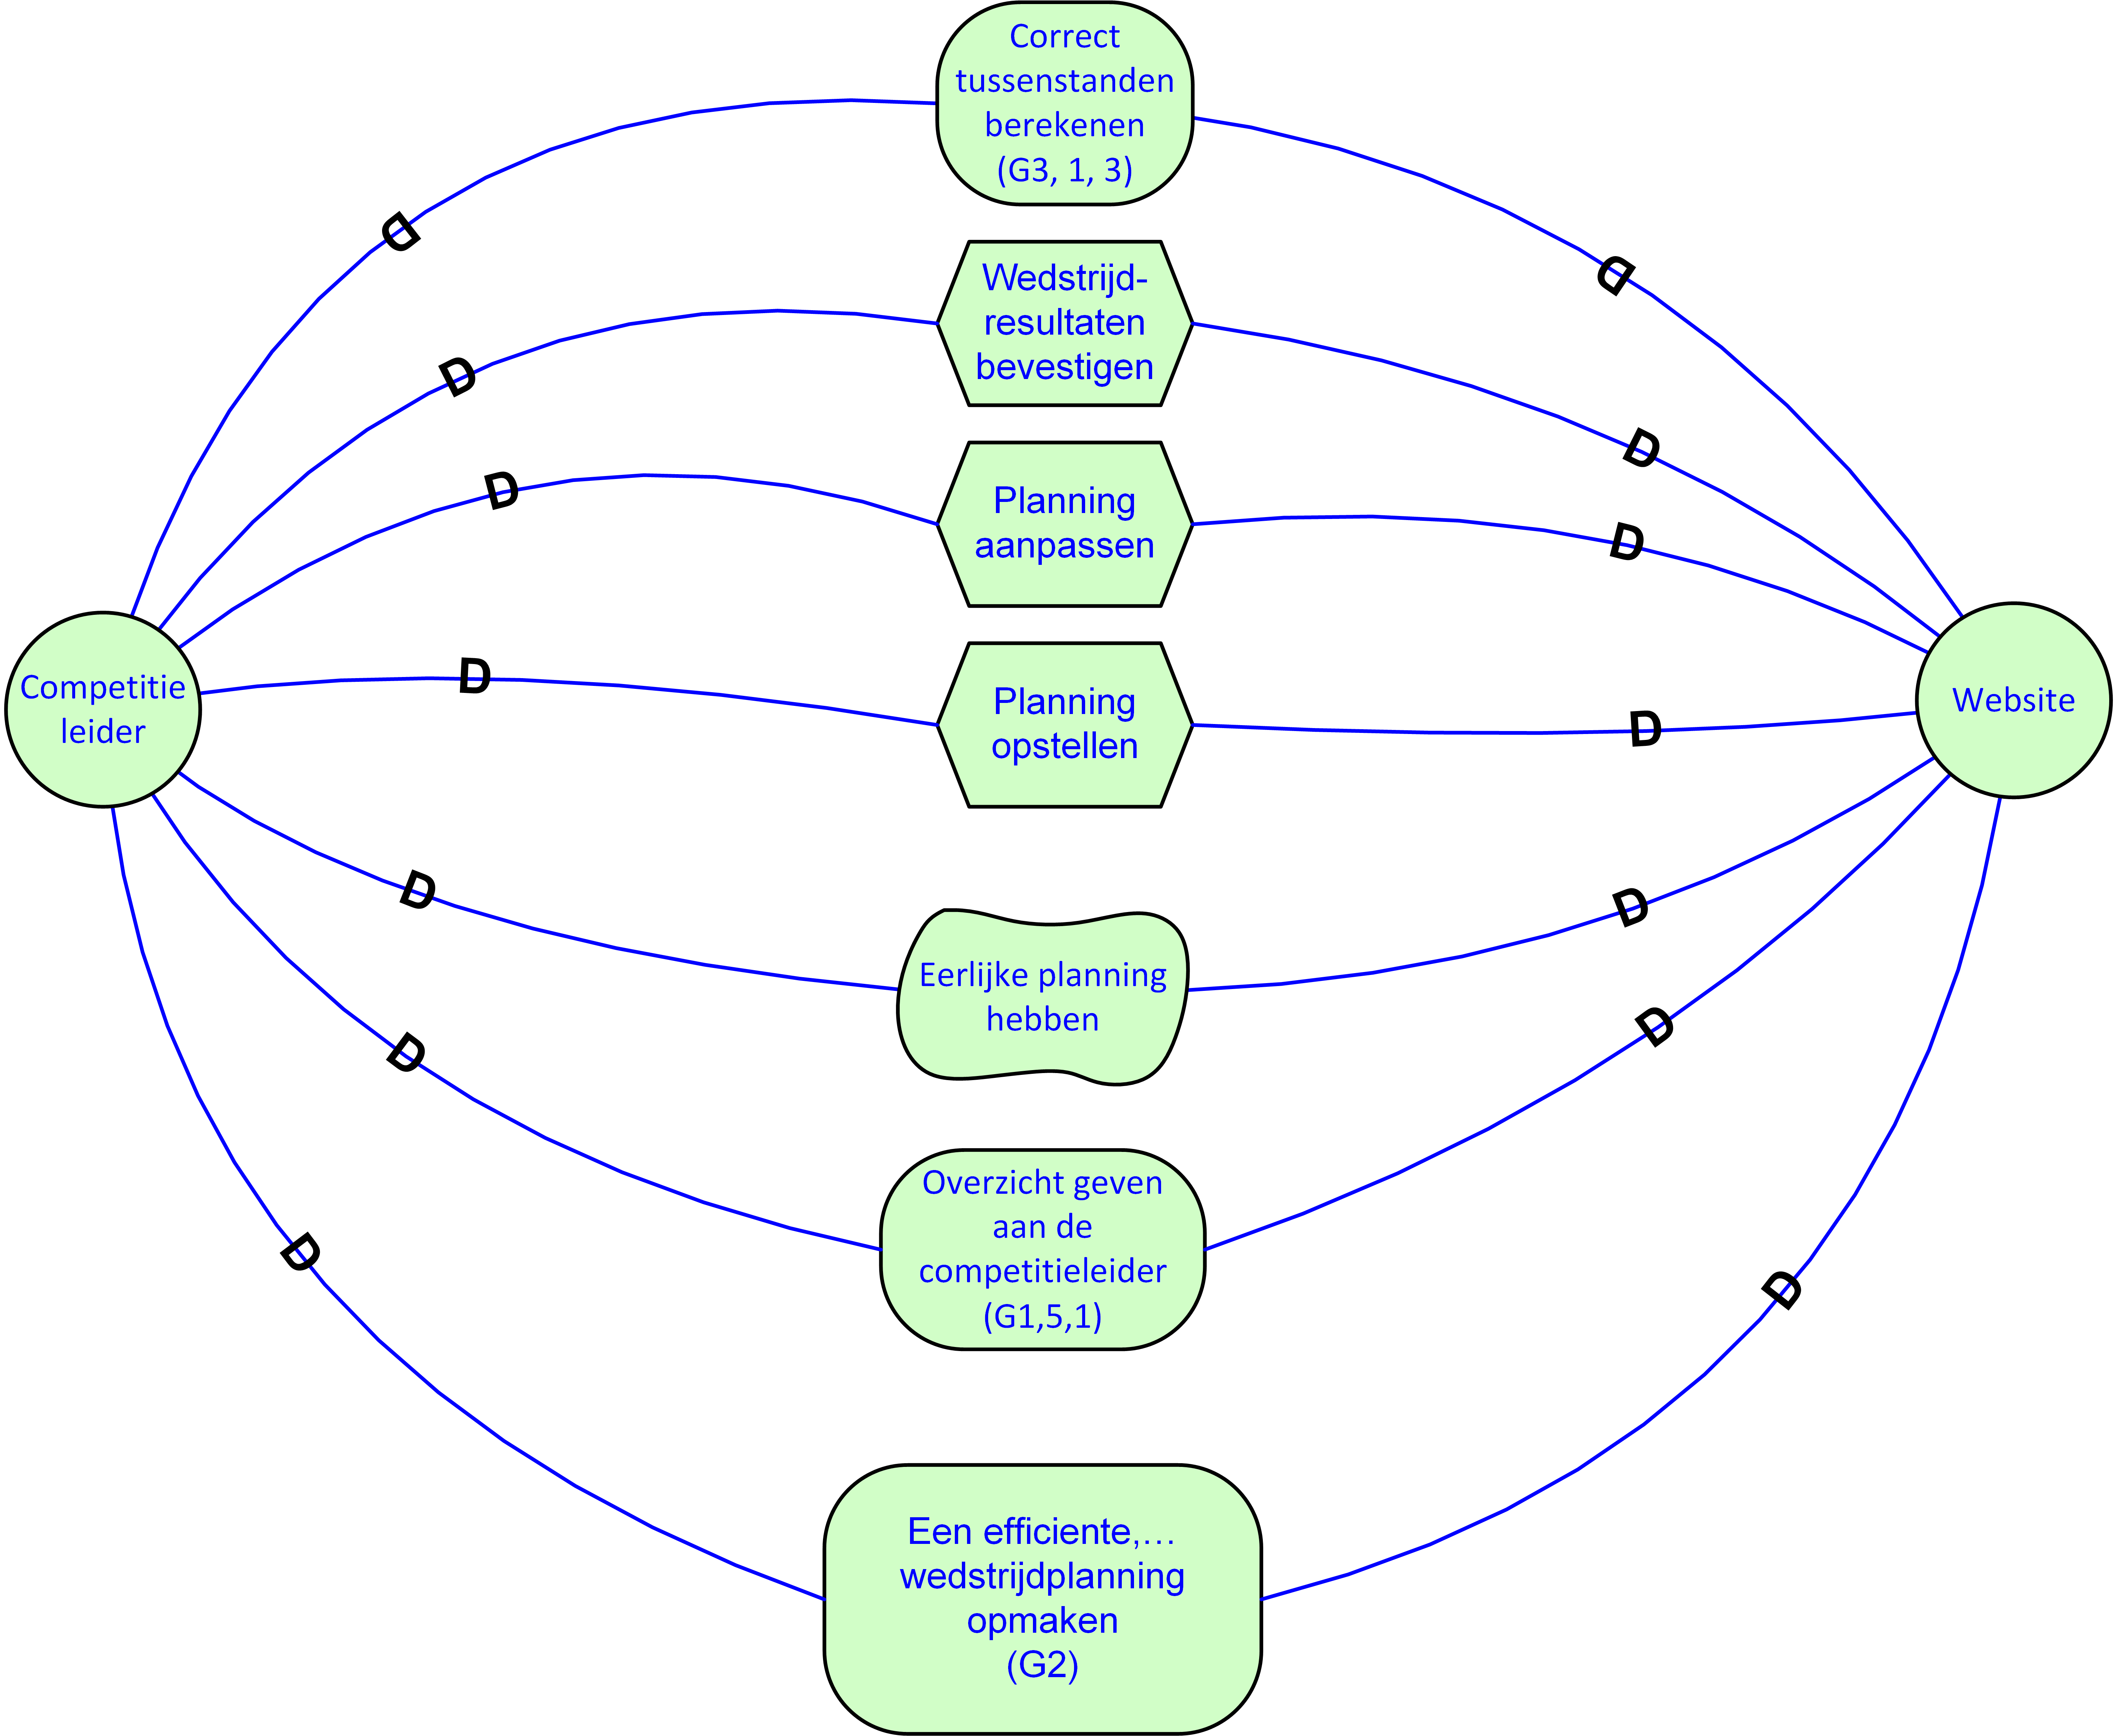
\includegraphics[width=\textwidth]{../2-Doelen/istar1.png}
			\caption{Eerste Dependency model in i*}
			\end{figure}
			\begin{figure}[H]
				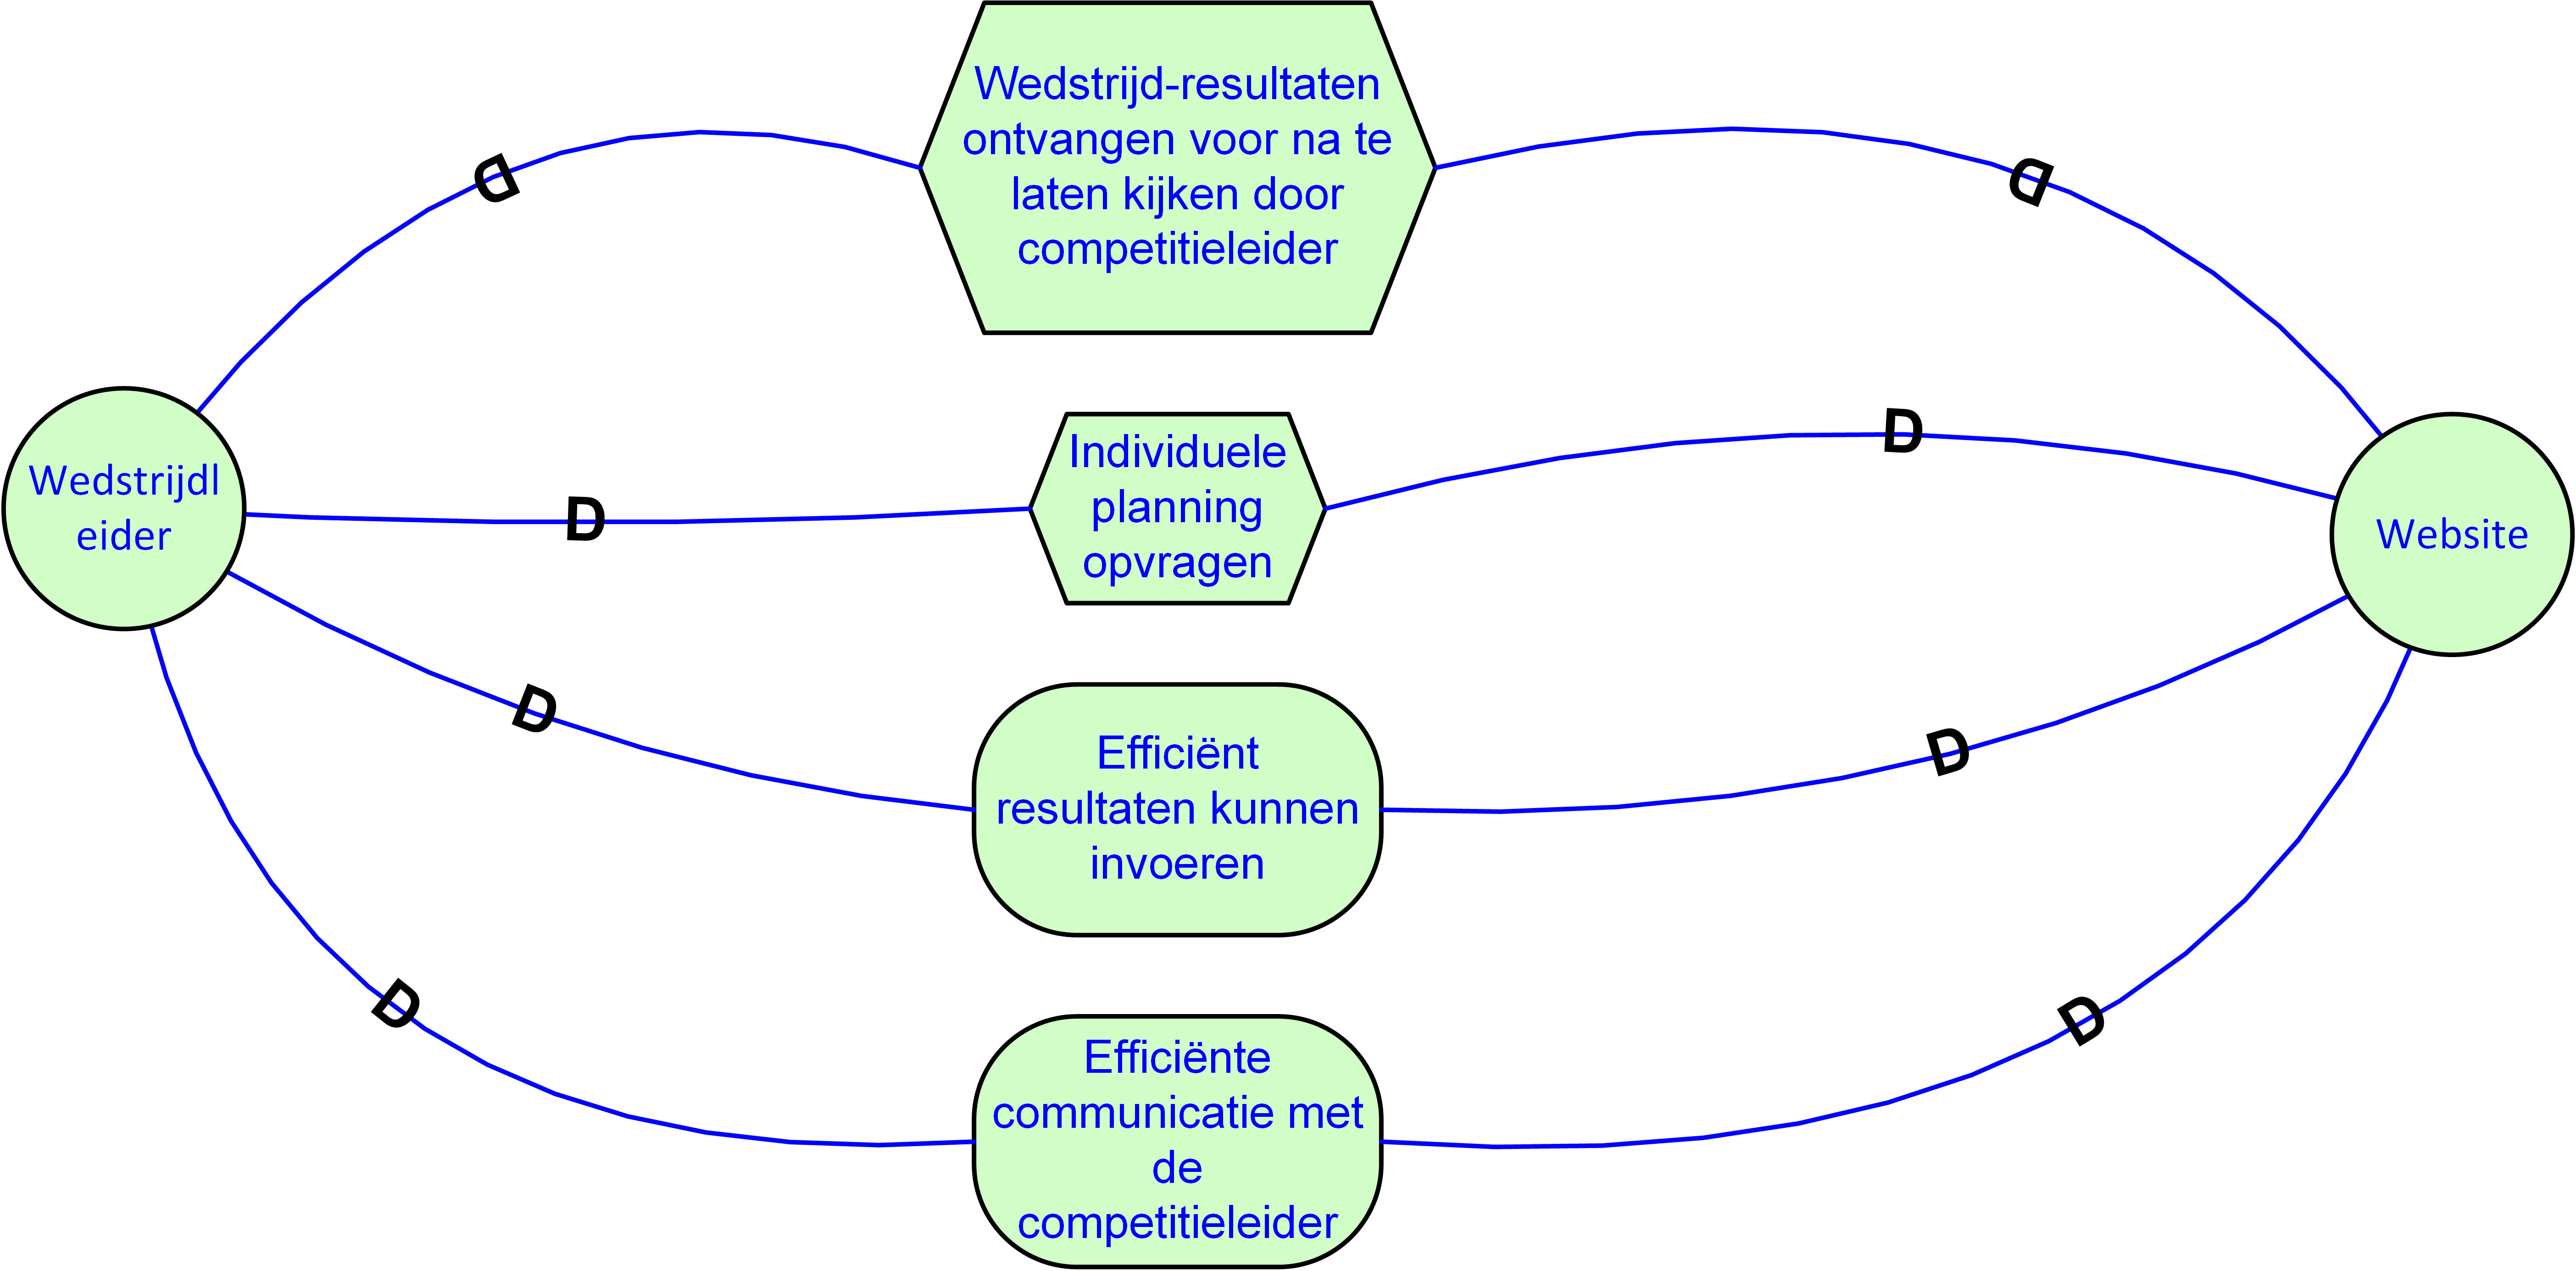
\includegraphics[width=\textwidth]{../2-Doelen/istar2.png}
				\caption{Tweede Dependency model in i*}
			\end{figure}
			\begin{figure}[H]
				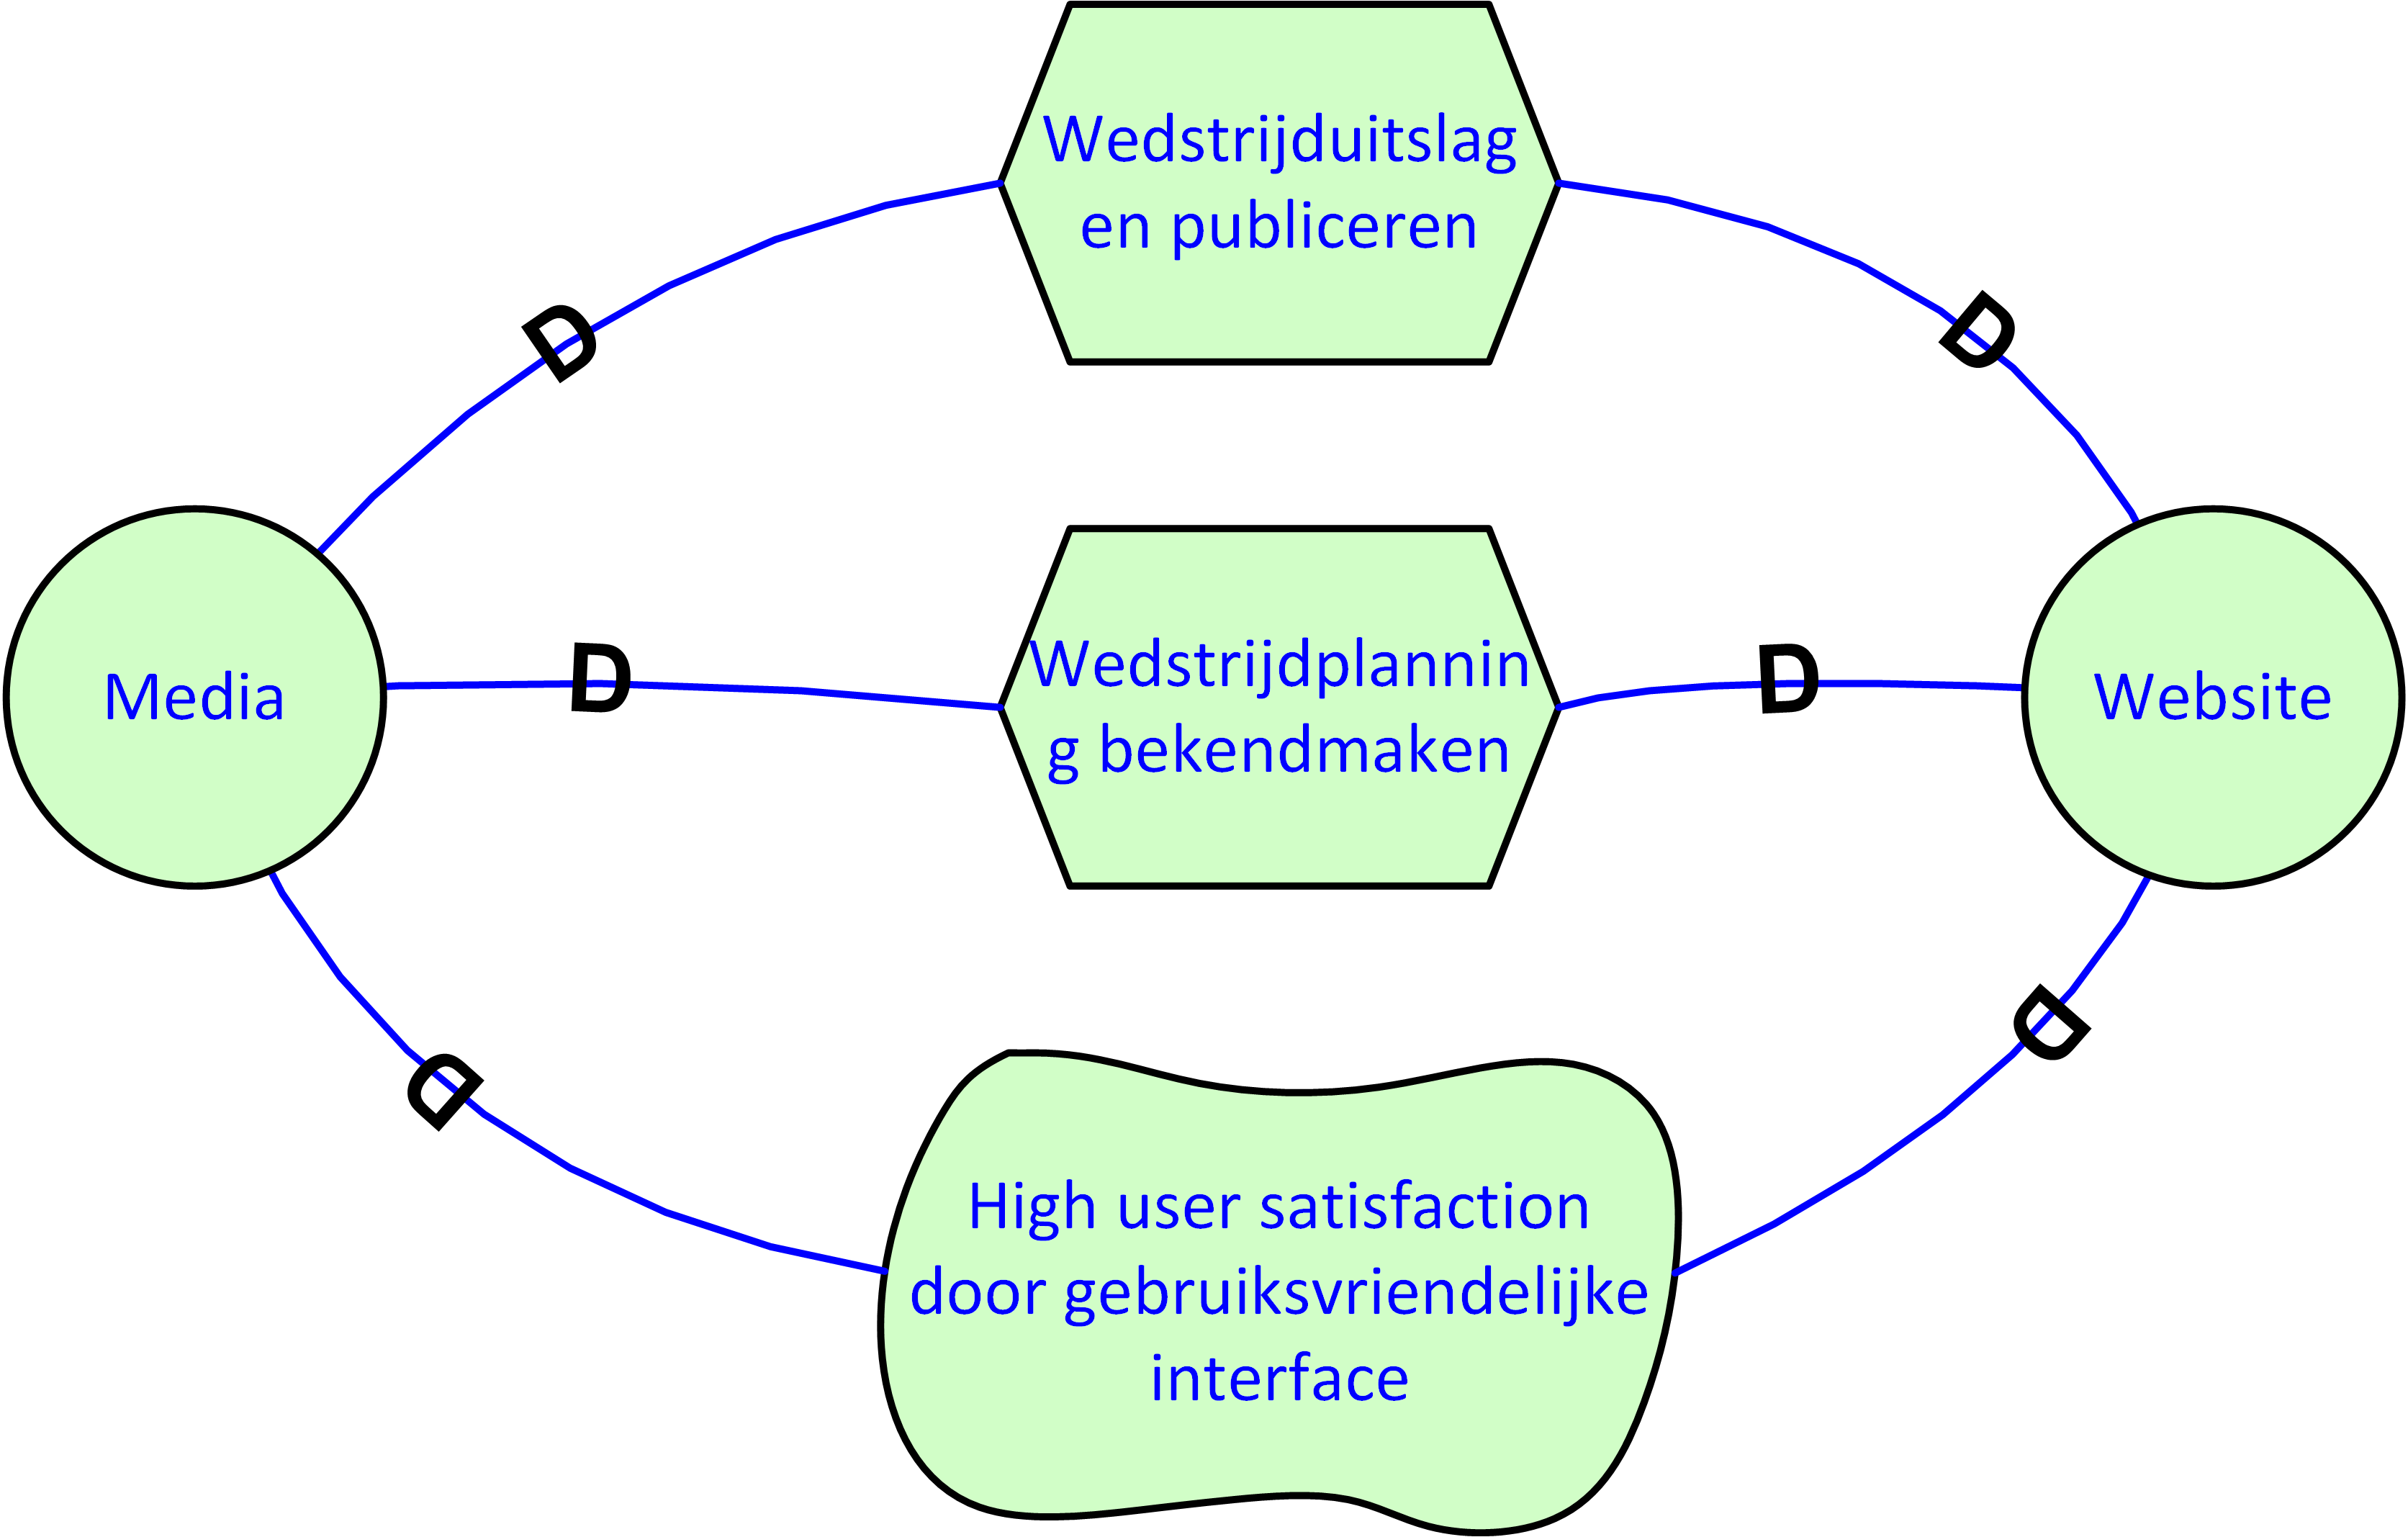
\includegraphics[width=\textwidth]{../2-Doelen/istar3.png}
				\caption{Derde Dependency model in i*}
			\end{figure}
			\subsection{Rationale}
			\begin{figure}[H]
				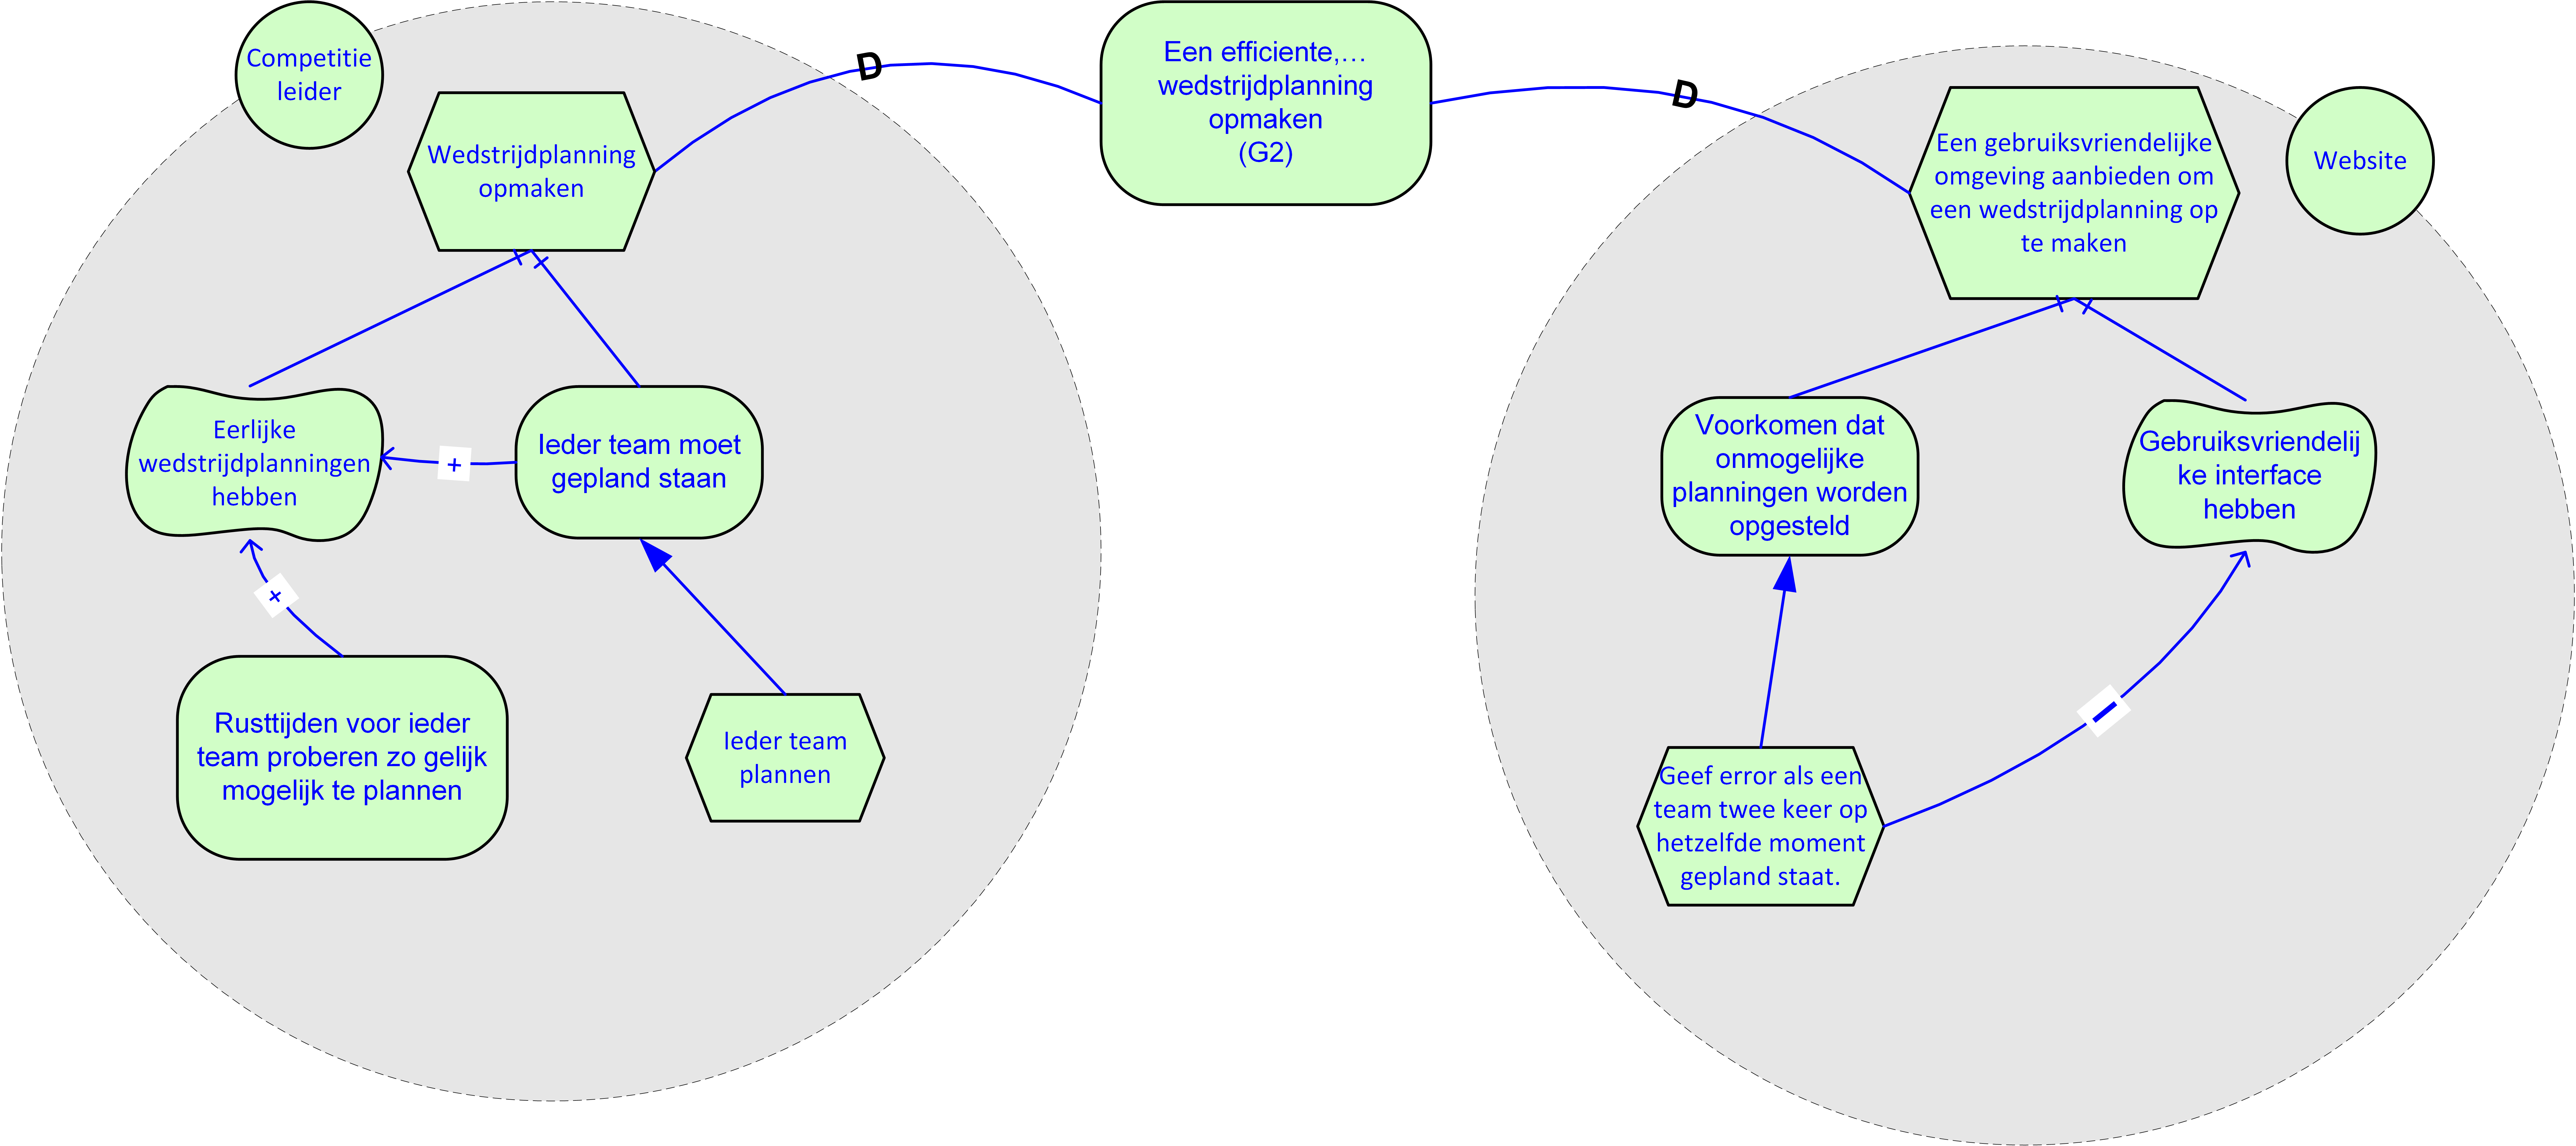
\includegraphics[width=\textwidth]{../2-Doelen/istar4.png}
				\caption{Strategic Rationale model in i*}
			\end{figure}
		\section{Scenarios}
			\subsection{``Planning opstellen''}
			De competitieleider wil een nieuwe match tussen 2 ploegen in de planning zetten. Hij gaat naar de website, drukt op “log in” en voert zijn persoonlijke inloggegevens in. De competitieleider heeft de optie om de wedstrijdplanning aan te passen of een nieuwe match toe te voegen op de website. Hij gaat naar de webpagina waar hij een nieuwe wedstrijd kan toevoegen via de knop “wedstrijd toevoegen”. Vervolgens krijgt hij een overzicht van de beschikbaarheden van de ploegen, plaatsen, tijdstippen, shoutcasters, scheidsrechters. (Hij ziet een paar velden waar hij de naam van de ploegen, de plaats, het tijdstip, de scheidsrechter en de shoutcasters nodig voor de match kan invullen.) Hij vult de namen van de 2 ploegen in die hij tegen elkaar wilt laten spelen. Hij selecteert een plaats tussen de mogelijkheden opgeslagen in de database. De competitieleider voegt vervolgens een beschikbaar tijdstip toe, alsook een scheidsrechter uit de database die op het gegeven tijdstip beschikbaar is. De competitieleider wijst ook shouters toe voor de wedstrijd. De competitieleider slaat de nieuwe gegevens op en sluit de website.
			\newpage
			\subsection{``Planning updaten''}
			\begin{enumerate}
				\item De competitieleider opent de website
				\item De competitieleider drukt op ``log in''
				\item De competitieleider meldt zich aan met zijn persoonlijke inloggegevens
				\item De competitieleider klikt op de knop ``wedstrijdplanning aanpassen''
				\item De competitieleider klikt op de knop ``alle geplande wedstrijden weergeven''
				\item De competitieleider klikt op de planning die hij wilt aanpassen
				\item De competitieleider klikt op de knop ``invoeren ploegnaam''
				\item De competitieleider voert de naam van de ploeg in, in het veld ``Ploegnaam''
				\item De competitieleider klikt op de knop ``wijzigingen opslaan''
				\item De competitieleider klikt op de knop ``afmelden''
				\item De competitieleider sluit de competitiewebsite
			\end{enumerate}
			\subsection{``Planning wijzigen''}
			De competitieleider probeert op de planning op de website een timeslot te wijzigen dat al voorbij is:
			\begin{enumerate}
				\item De competitieleider opent de website
				\item De competitieleider drukt op “log in” 
				\item De competitieleider meldt zich aan met zijn persoonlijke inloggegevens
				\item De competitieleider klikt op de knop ``wedstrijdplanning aanpassen'' 
				\item De competitieleider klikt op de knop ``alle geplande wedstrijden weergeven''
				\item De competitieleider klikt op de planning die hij wilt aanpassen
				\item De competitieleider klikt op de knop ``wijzig tijdstip''
				\item De competitieleider klikt op een timeslot dat reeds voorbij is.
				\item Er opent een waarschuwingsvenster waar opstaat: 'dit timeslot kan niet aangepast worden: datum is al voorbij'.
				\item De planning blijft onveranderd.
			\end{enumerate}
			\subsection{``Ploeg aanmaken''}
			Parth Naidu, de coach van ploeg Team SoloMid, wilt Sneaky, een speler van ploeg Cloud 9, toevoegen aan zijn team:
			\\
			Parth Naidu, de coach van ploeg Team SoloMid, opent de website. Hij klikt op ``log in'' en logt vervolgens in met zijn persoonlijke inloggegevens. Vervolgens ziet hij een link naar ``ploegen beheren'', waar hij dan ook op klikt. De site brengt hem dan naar een pagina waar hij zijn ploeg kan beheren, op die pagina staat ook een link om een speler toe te voegen. Hij klinkt op deze link en krijgt vervolgens een formulier dat hij kan invullen om een nieuwe speler aan zijn ploeg toe te voegen. Hij vult de gegevens van Sneaky, een speler van ploeg Cloud 9, in op het formulier. Hij probeert dit ingevulde formulier in te vullen. De website weigert deze verandering door te voeren en laat een waarschuwing zien aan Parth Naidu, waar op staat: ``Deze speler speelt al voor een andere ploeg, hij mag niet voor 2 ploegen tegelijk spelen. Hij moet eerst de andere ploeg verlaten vooraleer hij bij een andere ploeg kan toegevoegd worden.''
			\section{Datamodel}
				\subsection{UML diagram}
				\begin{figure}[H]
					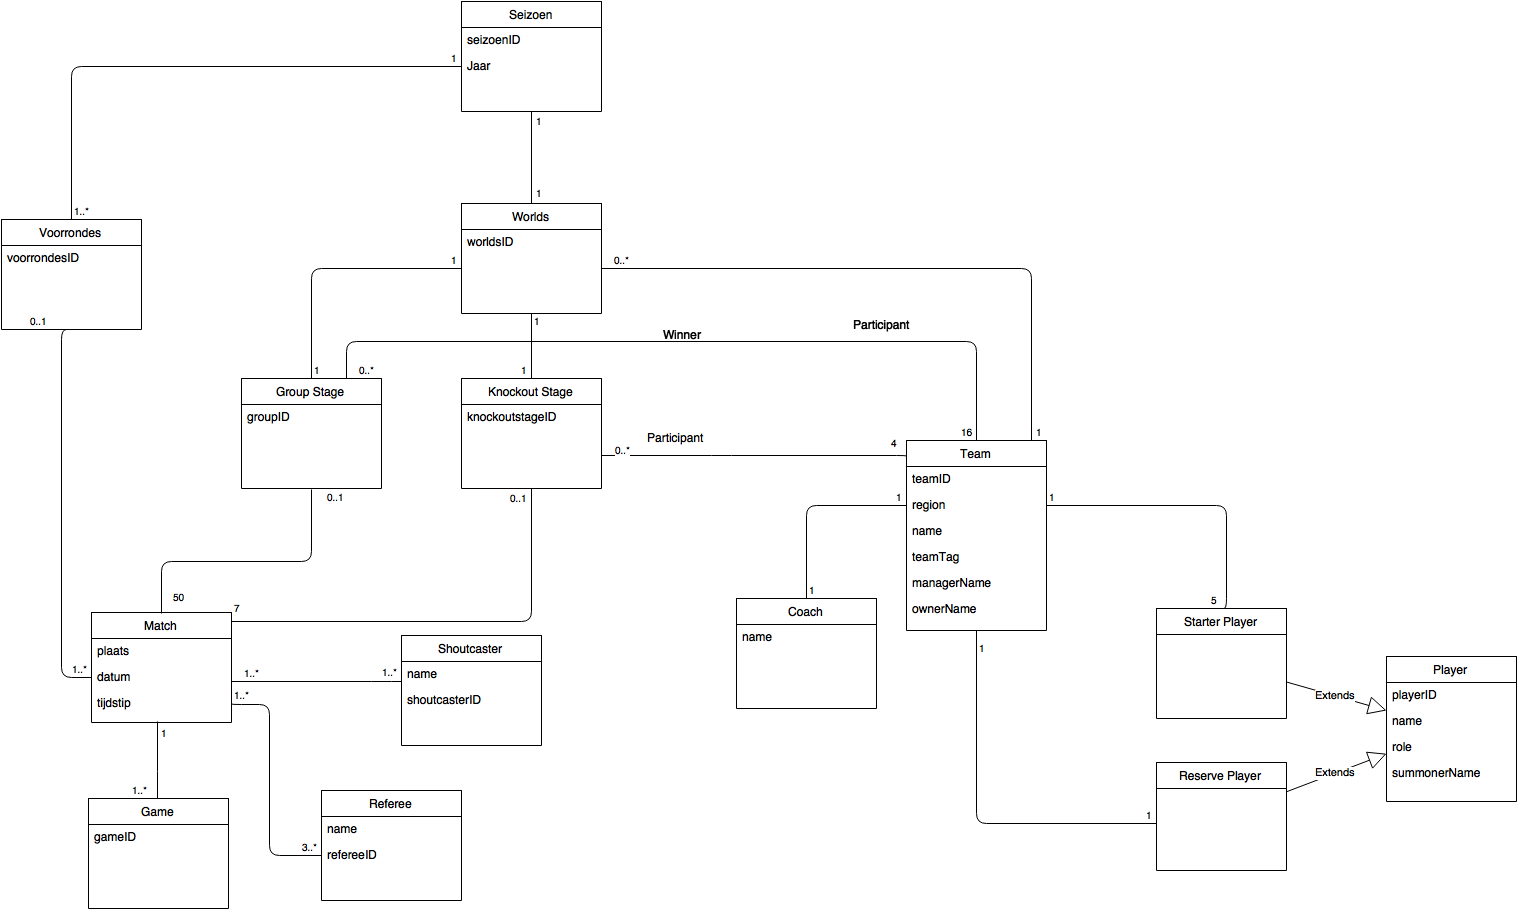
\includegraphics[width=\textwidth]{../4-Datamodel/RE.png}
					\caption{UML representatie van het model}
				\end{figure}
				\subsection{OCL Constraints}
\begin{lstlisting}[frame=single, language=OCL]
context Worlds invariant
group_stage.Participant ->
	includesAll(knockout_stage.participant)
\end{lstlisting}
Alle teams van de knockout stage moeten ook aan de group stage hebben meegedaan. \\

\begin{lstlisting}[frame=single, language=OCL]	
context Worlds invariant
Knockout_stage.Participant -> includesAll(winner)
\end{lstlisting}
De winnaar van worlds moet hebben meegedaan in de knockout stage. \\

\begin{lstlisting}[frame=single, language=OCL]
context Team invariant
starter_player -> excludeAll(reserve_player)
\end{lstlisting}
Een speler is oftewel een starter player oftewel een reserve player, hij kan niet beide tegelijk zijn. \\

	\section{State machine}
\end{document}